\documentclass[]{article}

% Imported Packages
%------------------------------------------------------------------------------
\usepackage{amssymb}
\usepackage{amstext}
\usepackage{amsthm}
\usepackage{amsmath}
\usepackage{enumerate}
\usepackage{fancyhdr}
\usepackage[margin=1in]{geometry}
\usepackage{graphicx}
%\usepackage{extarrows}
%\usepackage{setspace}
%\usepackage{xcolor}
\usepackage{color}
\usepackage{parskip}
\usepackage{comment}
\usepackage{enumitem}
\usepackage{hyperref}
%------------------------------------------------------------------------------

% Header and Footer
%------------------------------------------------------------------------------
\pagestyle{plain}  
\renewcommand\headrulewidth{0.4pt}                                      
\renewcommand\footrulewidth{0.4pt}                                    
%------------------------------------------------------------------------------

% Title Details
%------------------------------------------------------------------------------
\title{Deliverable \#1: Software Requirement Specification (SRS)}
\author{SE 3A04: Software Design II -- Large System Design}
\date{}
                            
%------------------------------------------------------------------------------

% Document
%------------------------------------------------------------------------------
\begin{document} 

\maketitle	
\noindent{\bf Tutorial Number:} T03\\
{\bf Group Number:} G8 \\
{\bf Group Members:} Hashim Bukhtiar, Jaden Moore, James Ariache, Olivia Reich, Omar Abdelhamid
\begin{itemize}
        \item Hashim Bukhtiar
        \item Jaden Moore
        \item James Ariache
        \item Olivia Reich
        \item Omar Abdelhamid
\end{itemize}

\section*{IMPORTANT NOTES}
\begin{itemize}
	\item Be sure to include all sections of the template in your document regardless whether you have something to write for each or not
	\begin{itemize}
		\item If you do not have anything to write in a section, indicate this by the \emph{N/A}, \emph{void}, \emph{none}, etc.
	\end{itemize}
	\item Uniquely number each of your requirements for easy identification and cross-referencing
	\item Highlight terms that are defined in Section~1.3 (\textbf{Definitions, Acronyms, and Abbreviations}) with \textbf{bold}, \emph{italic} or \underline{underline}
	\item For Deliverable 1, please highlight, in some fashion, all (you may have more than one) creative and innovative features. Your creative and innovative features will generally be described in Section~2.2 (\textbf{Product Functions}), but it will depend on the type of creative or innovative features you are including.
\end{itemize}

\newpage
\section{Introduction}
\label{sec:introduction}
The SRS is a structured document that outlines the functional and non-functional requirements of the RideRecon software system. It serves as a blueprint for developers, testers, and stakeholders, ensuring a clear understanding of the system to be built. This SRS will provide visibility over software requirements for RideRecon, a taxi rideshare application. 
This document will discuss the purpose of RideRecon, the scope of the application, user characteristics, product requirements, and use case diagrams.


\subsection{Purpose}
\label{sub:purpose}
The document focuses on software requirements, user characteristics, and use cases for RideRecon.
The purpose of this SRS is to define the software’s objectives, scope, and functionalities. This document is intended for internal RideRecon stakeholders, including but not limited to, project managers, developers, domain experts, and RideRecon team members/investors. No prior readings are required.

\subsection{Scope}
\label{sub:scope}

RideRecon, the car identification application, will allow users to upload an image and text about a vehicle that they want to identify, consulting up to four “Experts” who will use all or some of the user’s input to determine the make and model of the car that has been depicted.

Users are required to register an account on RideRecon in order to access the car identification service. The service includes four experts: “RIS”, “G8M”, “4oE” and ”vAI”. The “RIS” expert performs a reverse image search with the user’s given image to identify the car. The “G8M” expert is a trained machine learning model by the developers that utilizes an optimized database of car images and their corresponding makes and models to identify the user’s car. The ”4oE” expert is the Large Language Model GPT-4o-mini, accessed through OpenAI’s API, which will utilize both the image and the text description to identify the car. Finally, the “vAI” expert is also an LLM, this one hosted on Google Cloud Platform using Vertex AI, specifically the Gemini 1.0 Flash Model, also accessed through its API.

RideRecon’s objective is not only to identify users’ vehicles, but also to deliver other innovative and creative features. For example, once the car has been identified, 4oE will provide an interesting fact about the car, adding more depth and intrigue to it, as well as provide sources and listings for where to purchase the car, allowing the user to go one step further and save time if they are interested in making that vehicle their own.

One of the goals of the software is to increase users, as more users will lead to more cars being identified and added to the optimized database of G8M, and thus better car identification overall, which is even better for future users. Another goal would be to to monetize its user base by offering premium features like better expert access, exclusive community forums, or partnerships with car-related businesses, thereby creating additional revenue streams beyond the core car identification service. This diversification will improve long-term sustainability and profitability.


\subsection{Definitions, Acronyms, and Abbreviations}
\label{sub:definitions_acronyms_and_abbreviations}
\textbf{LLM}: Large Language Model. A sophisticated artificial intelligence that can understand, generate, and translate human language, often used for tasks like text generation, question answering, and translation.

\textbf{RIS}: Reverse Image Search. This is the idea of using an image as a search query in a browser to find results, rather than using text as traditional browser searches as performed.

\textbf{G8M}: Group 8 Model. This is the model trained by the developers of RideRecon to identify cars. It will utilize an optimized dataset of car images and makes and models.

\textbf{4oE}: GPT-4o-mini. This is an LLM that uses text and images to determine the make and model of the user's car.

\textbf{vAI}: Vertex AI, Gemini 1.0 Flash. This is the LLM that uses images to determine the make and model of the user's car.

\textbf{Finalizer}: The component of the system that consolidates and finalizes the output, including resolving conflicts between experts and outputting the fun fact about the car and where to purchase it.

\subsection{References}
\label{sub:references}
% Begin SubSection
\begin{itemize}
    \item Provide a complete list of all documents referenced elsewhere in the SRS.
    \item Identify each document by title, report number (if applicable), date, and publishing organization.
    \item Specify the sources from which the references can be obtained.
    \item Order this list in some sensible manner (alphabetical by author, or something else that makes more sense).
\end{itemize}

\begin{itemize}
    \item \url{https://play.google.com/store/apps/details?id=ru.egoroffsoft.avtopix&hl=en_CA&pli=1}
    \item \url{https://play.google.com/store/apps/details?id=com.mm999.car&hl=en_CA}
\end{itemize}

% End SubSection

\subsection{Overview}
\label{sub:overview}

\textbf{Section 2} discusses the overall product description talking about the product perspective, product functions, user characteristics, assumptions and dependencies, and apportioning of requirements. 

\textbf{Section 3} contains the Use Case Diagram for the use case scenario of creating a carpool. 

\textbf{Section 4} contains the highlights of functional requirements talking about main business events and viewpoints. 

\textbf{Section 5} contains the Non-Functional Requirements talking about Look and Feel Requirements, Usability and Humanity Requirements, Performance Requirements, Operational and Environmental Requirements, Maintainability and Support Requirements, Security Requirements, Cultural and Political Requirements and Legal Requirements. 

Lastly, \textbf{Section A} contains the Division of Labour.


% End Section
\newpage
\section{Overall Product Description}
\label{sec:overall_description}
% Begin Section
\begin{comment}
\begin{itemize}
	\item This section should describe the general factors that affect the product and its requirements. 
	\item It does not state specific requirements.
	\item It provides a \emph{background} for those requirements and makes them easier to understand.
\end{itemize}
\end{comment}

\subsection{Product Perspective}
\label{sub:product_perspective}
% Begin SubSection
\begin{comment}
\begin{itemize}
	\item Put the product into perspective with other related products, i.e., context
	\item If the product is independent and totally self-contained, it should be stated here
	\item If the SRS defines a product that is a component of a larger system, then this subsection should relate the requirements of that larger system to the functionality of the software being developed. Identify interfaces between that larger system and the software to be developed.
	\item A block diagram showing the major components of the larger system, interconnections, and external interfaces can be helpful
\end{itemize}
\end{comment}

RideRecon is a mobile app for car identification that is developed to be compatible with the Android platform.Similar to products such as AvtoPix [insert reference] and CarsSnap [insert reference], it will allow car identification through images while also enhancing search capabilities by also allowing identification through textual descriptions. The product will allow users to create a profile and edit account information linked to that profile. This includes the creation of virtual car collections using car images submitted in the app.

Once an image is selected by the user, the product will have an interface that allows it to interact with different reverse image search technologies. Specifically, it will be able to access a Vertex AI image model and the Reverse Image Search Tool via Google.

If provided textual input by the user, the product will have an interface to interact with Google Search. This interface will also be used to search for relevant car facts that can be returned to the user upon identifying pivotal car identification information.

\begin{center}
	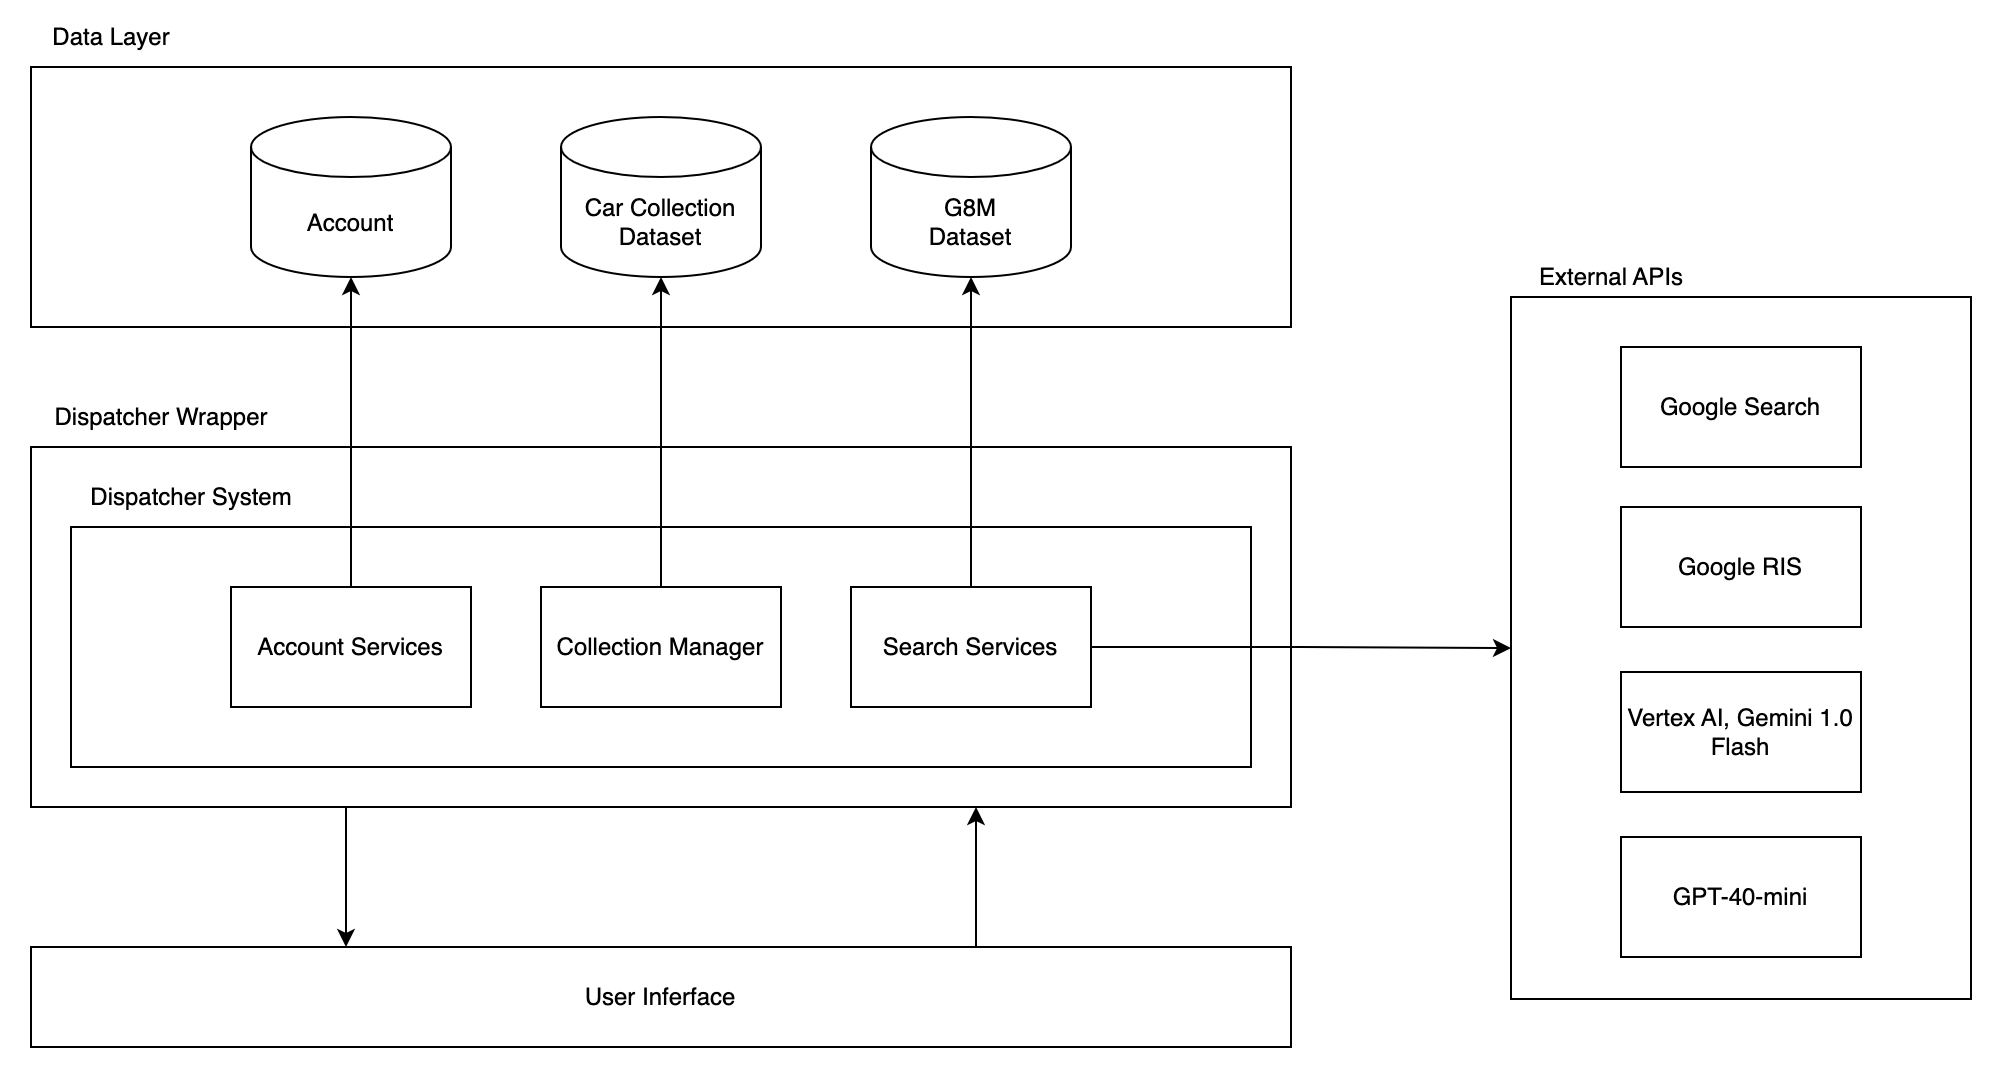
\includegraphics[width=0.9\textwidth]{images/system_diagram.png} \\
	\textbf{Figure 1. } System Diagram
\end{center}

% End SubSection

\newpage
\subsection{Product Functions}
\label{sub:product_functions}
% Begin SubSection
\begin{comment}
\begin{itemize}
	\item Provide a \emph{summary} of the major functions that the software will perform.
	\begin{itemize}
		\item \textbf{Example}: An SRS for an accounting program may use this part to address customer account maintenance, customer statement, and invoice preparation without mentioning the vast amount of detail that each of those functions requires.
	\end{itemize}
	\item Functions should be organized in a way that makes the list of functions understandable to the customer or to anyone else reading the document for the first time 
	\item Present the functions in a list format - each item should be one function, with a brief description of it
	\item Textual or graphical methods can be used to show the different functions and their relationships
	\begin{itemize}
		\item Such a diagram is not intended to show a design of a product, but simply shows the logical relationships among variables
	\end{itemize} 
\end{itemize}
\end{comment}

There will be 3 modules in the product. Each module focuses on different major functions within the product, which have been defined in the table below.

\begin{tabular}{|p{3cm}|p{13cm}|}
	\hline
	Modules & Functions \\
	\hline
	Account Services &
	\begin{itemize} [left=2pt]
		\item Create an account
		\item Login and logout of account
		\item Update account information
		\item Account recovery
		\begin{itemize}
			\item allow user to reset password if forgotten
		\end{itemize}
		\item Authenticate account
		\begin{itemize}
			\item verifies contact information only done during account creation or recovery
		\end{itemize}
	\end{itemize} \\
	\hline
	Search Services &
	\begin{itemize} [left=2pt]
		\item Image search
		\begin{itemize}
			\item allow user to request car identification through an image
		\end{itemize}
		\item Text search
		\begin{itemize}
			\item allow user to request car identification through  text descriptors
		\end{itemize}
		\item Present car information
		\begin{itemize}
			\item displays all relevant identification information
			\item displays ‘fun fact’ information
		\end{itemize}
		\item Confirm car identification
		\begin{itemize}
			\item allow user to confirm whether the identified information matches the car
		\end{itemize}
		\item Add car to collection
		\begin{itemize}
			\item allow user to add identified car to specified ‘Car Collection’
		\end{itemize}
	\end{itemize} \\
	\hline
	Collection Manager &
	\begin{itemize} [left=2pt]
		\item Create new collection
		\begin{itemize}
			\item allow user to create new sub-class in their car collection
		\end{itemize}
		\item View collection
		\begin{itemize}
			\item allow user to select and view a car collection
		\end{itemize}
	\end{itemize} \\
	\hline
\end{tabular}

\begin{center}
	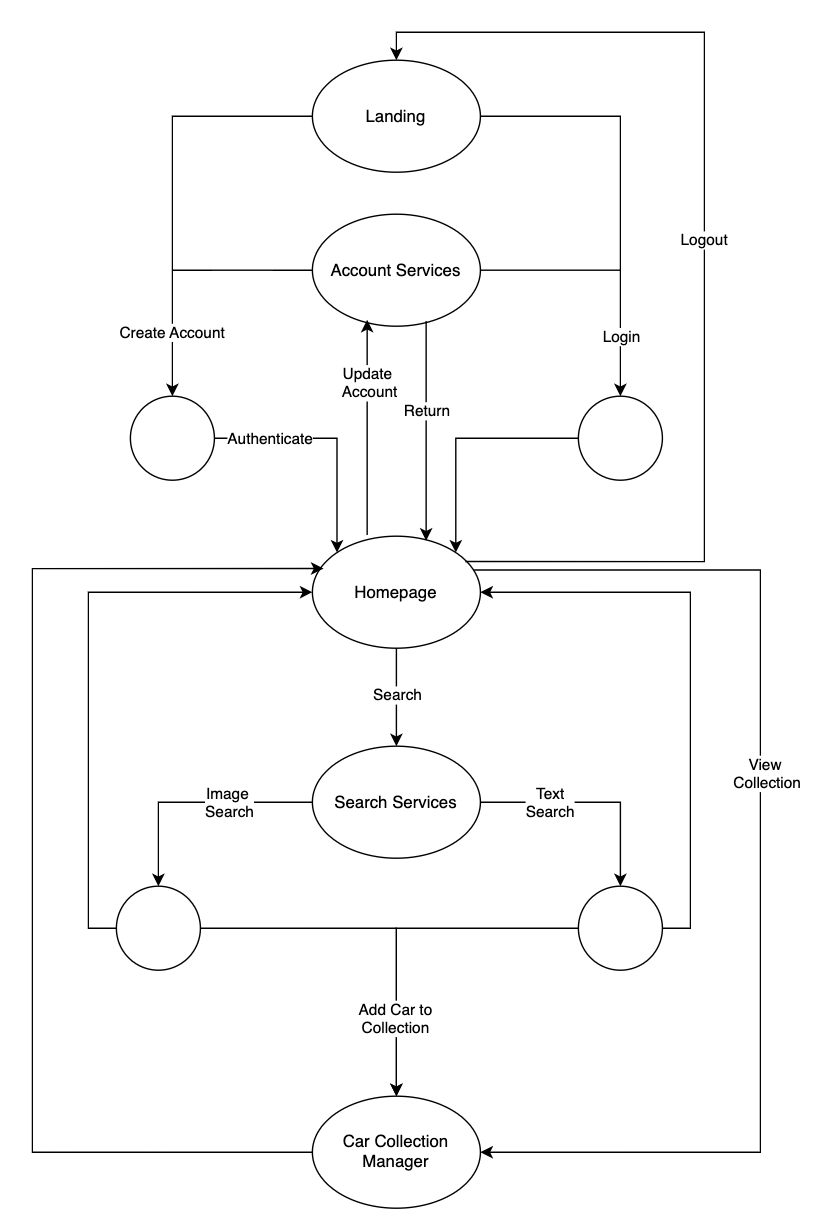
\includegraphics[width=0.5\textwidth]{images/state_diagram.png} \\
	\textbf{Figure 2. } State Diagram
\end{center}
% End SubSection

\subsection{User Characteristics}
\label{sub:user_characteristics}
% Begin SubSection
\begin{comment}
\begin{itemize}
	\item Describe those general characteristics of the intended users of the product including educational level, experience, and technical expertise 
	\item Since there will be many users, you may wish to divide into different user types or personas
%	\item Do not state specific requirements, but rather provide the reasons why certain specific requirements are later specified
\end{itemize}
\end{comment}
\begin{itemize}
	\item \textbf{Educational Level:} Users must have basic literacy skills which includes the fundamental ability to understand information through reading, writing, listening, and speaking.
	\item \textbf{Technical Expertise:} Users should have a basic understanding of how to operate and navigate an Android smartphone, including downloading apps, as this application is designed specifically for the Android platform.
	\item \textbf{Technical Experience:} Users do not require any prior experience or knowledge with cars in order to utilize the app. Aside from the basic technical expertise outlined above, no extra experience will be required to navigate and utilize the features of the app as it will prioritize an intuitive design.
\end{itemize}
% End SubSection

\subsection{Constraints}
\label{sub:constraints}
% Begin SubSection
\begin{itemize}
	\item Provide a general description of any constraints that will limit the developer's options
	
	\item The system must have an active \textbf{internet connection} to perform car identification.
    \item The app must be compatible with \textbf{Android 8.0 (Oreo) and above}.
    \item The device must have at least \textbf{2GB of RAM} for smooth operation.
    \item Captured images must have a \textbf{minimum resolution of 720p} to ensure accurate car identification.
    \item The AI model may not recognize \textbf{damaged or heavily modified cars} accurately.
    \item The system must comply with \textbf{privacy laws} regarding the storage and processing of user-uploaded images.

\end{itemize}
% End SubSection

\subsection{Assumptions and Dependencies}
\label{sub:assumptions_and_dependencies}
% Begin SubSection
\begin{itemize}
	\item List any assumptions you made in interpreting what the software being developed is aiming to achieve
	\item List any other assumptions you made that, if it fails to hold, could require you to change the requirements
	%\item List each of the factors that affect the requirements stated in the SRS
	%\item These factors are not design constraints on the software but are, rather, any changes to them that can affect the requirements in the SRS
	\begin{itemize}
		\item \textbf{Example}: An assumption may be that a specific operating system will be available on the hardware designated for the software product. If, in fact, the operating system is not available, the SRS would then have to change accordingly.
	\end{itemize}

	\item \textbf{Assumptions:}
    \begin{itemize}
        \item Users will have stable internet access while using the app.
        \item The AI model can identify most common car brands and models.
        \item Dealerships will provide accurate and up-to-date pricing.
    \end{itemize}
    \item \textbf{Dependencies:}
    \begin{itemize}
        \item The AI model relies on an external \textbf{machine learning API} to process images.
        \item The system depends on a third-party \textbf{reverse image search API} (e.g., Google Lens, TinEye) for validation.
        \item Pricing and specifications are sourced from \textbf{external dealership databases}.
    \end{itemize}

\end{itemize}
% End SubSection

\subsection{Apportioning of Requirements}
\label{sub:apportioning_of_requirements}
% Begin SubSection
\begin{itemize}
	\item Identify requirements that may be delayed until future versions of the system
	\item \textbf{Offline Mode}: The app currently requires internet access; an offline model will be explored in future versions.
    \item \textbf{Multiple Car Detection}: Initially, the app will support one car per image; future updates may allow multiple cars.
    \item \textbf{Personalized Car Recommendations}: The first version won’t suggest similar cars, but this may be added later.
\end{itemize}
% End SubSection

% End Section
\section{Use Case Diagram}
\label{sec:use_case_diagram}
% Begin Section
\begin{itemize}
	\item Provide the use case diagram for the system being developed.
	\item You do not need to provide the textual description of any of the use cases here (these will be specified under "Highlights of Functional Requirements").
%	\item Provide \emph{one} use case diagram for the most important Business Event.
%	\item The text of all use cases will be specified under "Highlights of Functional Requirements"
\end{itemize}

\begin{center}
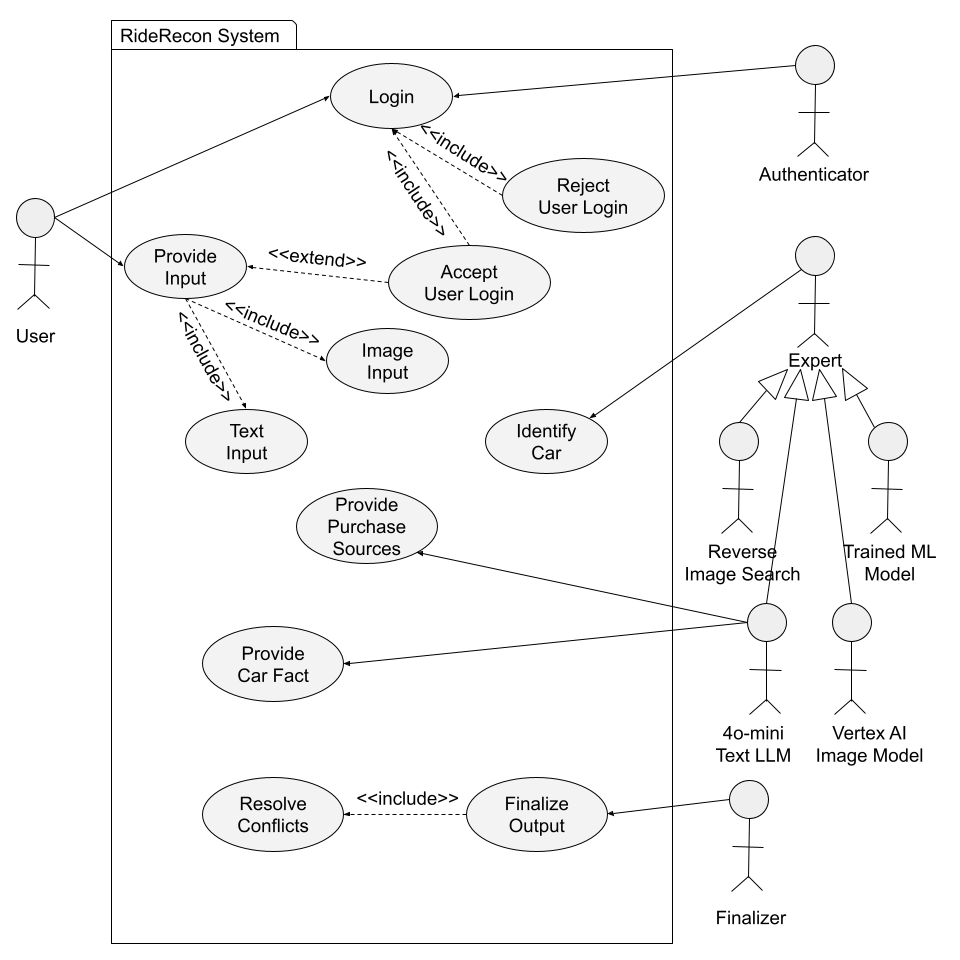
\includegraphics[height=13cm]{images/Use Case Diagram D1.png} \\
\textbf{Figure 3. } Use Case Diagram
\end{center}

%In this section, select the most important Business Event that your system responds to and give its use case diagram.  Only one use case diagram is needed.  Give a brief textual description of the use case without repeating what is in the scenarios of the corresponding Business Event.

%
%
%
%This section should provide a use case diagram for your application. 
%\begin{enumerate}[a)]
%	\item Each use case appearing in the diagram should be accompanied by a text description. 
%\end{enumerate}
%% End Section

\section{Highlights of Functional Requirements}
\label{sec:functional_requirements}
% Begin Section
\begin{itemize}
	\item Specify all use cases (or other scenarios triggered by other events), organized by Business Event. 
	\item For each Business Event, show the scenario from every Viewpoint. You should have the same set of Viewpoints across all Business Events. If a Viewpoint doesn't participate, write N/A so we know you considered it still. You can choose how to present this - keep in mind it should be easy to follow. 
	\item At the end, combine them all into a Global Scenario.
	%\item Specify the "use cases" (or other triggering events) organized by Business Event. (The Global Scenario is what you might think of as a use case). Be sure to consider Business Events that aren't just triggered by users with goals (e.g. something happens in the environment that your system needs to respond to)
	\item Your focus should be on what the system needs to do, not how to do it. Specify it in enough detail that it clearly specifies what needs to be accomplished, but not so detailed that you start programming or making design decisions.
	\item Keep the length of each use case (Global Scenario) manageable. If it's getting too long, split into sub-cases.
	\item You are \emph{not} specifying a complete and consistent set of functional requirements here. (i.e. you are providing them in the form of use cases/global scenarios, not a refined list). For the purpose of this project, you do not need to reduce them to a list; the global scenarios format is all you need.
	\item Red text below is just to highlight where you need to insert a scenario - don't actually write it all in red.
\end{itemize}

\noindent {\bf Main Business Events:} List out all the main business events you are presenting. If you sub-divided into smaller ones, you don't need to include the smaller ones in this list.\\
\begin{itemize}
        \item BE1. Create Account
        \item BE2. Authenticate User
        \item BE3. Upload Text and/or Image as Input
        \item BE4. Compare Expert Answers
        \item BE5. Present Final Output With Identification Information
        \item BE6. Add to or Remove From Car Collection
\end{itemize}

\noindent {\bf Viewpoints:} List out all the viewpoints you will be considering.\\
\begin{itemize}
	\item VP1. Users
	\item VP2. Customer Support (RideRecon)
	\item VP3. Marketing (RideRecon)
	\item VP4. Accounting (RideRecon)
	\item VP5. Dealership
\end{itemize}

\noindent {\bf Interpretation:} Specify any liberties you took in interpreting business events, if necessary.\\
\begin{itemize}
	\item NA.
\end{itemize}

\begin{enumerate}[label={\bf BE\arabic*.}]
	\item Create Account \#1
		\begin{enumerate}[label=\textbf{VP\arabic*.}]
			\item Users \#1 \\
				\textcolor{red}{Insert Scenario Here}
			\item Customer Support (RideRecon) \#2 \\
				\textcolor{red}{Insert Scenario Here}
			\item Marketing (RideRecon) \#3 \\
				\textcolor{red}{Insert Scenario Here}
			\item Accounting (RideRecon) \#4 \\
				\textcolor{red}{Insert Scenario Here}
			\item Dealership \#5 \\
				\textcolor{red}{Insert Scenario Here}
		\end{enumerate}
		{\bf Global Scenario:}\\
		\textcolor{red}{Insert Scenario Here}
	\item Authenticate User \#2
	\begin{enumerate}[label={\bf VP\arabic*.}]
		\item Users \#1 \\
			\textcolor{red}{Insert Scenario Here}
		\item Customer Support (RideRecon) \#2 \\
			\textcolor{red}{Insert Scenario Here}
		\item Marketing (RideRecon) \#3 \\
			\textcolor{red}{Insert Scenario Here}
		\item Accounting (RideRecon) \#4 \\
			\textcolor{red}{Insert Scenario Here}
		\item Dealership \#5 \\
			\textcolor{red}{Insert Scenario Here}
	\end{enumerate}
	{\bf Global Scenario:}\\
	\textcolor{red}{Insert Scenario Here}
	\item Upload Text adn Image as Input \#3
		\begin{enumerate}[label=\textbf{VP\arabic*.}]
			\item Users \#1 \\
				\textcolor{red}{Insert Scenario Here}
			\item Customer Support (RideRecon) \#2 \\
				\textcolor{red}{Insert Scenario Here}
			\item Marketing (RideRecon) \#3 \\
				\textcolor{red}{Insert Scenario Here}
			\item Accounting (RideRecon) \#4 \\
				\textcolor{red}{Insert Scenario Here}
			\item Dealership \#5 \\
				\textcolor{red}{Insert Scenario Here}
		\end{enumerate}
		{\bf Global Scenario:}\\
		\textcolor{red}{Insert Scenario Here}
	\item Compare Expert Answers \#4
	\begin{enumerate}[label={\bf VP\arabic*.}]
		\item Users \#1 \\
			\textcolor{red}{Insert Scenario Here}
		\item Customer Support (RideRecon) \#2 \\
			\textcolor{red}{Insert Scenario Here}
		\item Marketing (RideRecon) \#3 \\
			\textcolor{red}{Insert Scenario Here}
		\item Accounting (RideRecon) \#4 \\
			\textcolor{red}{Insert Scenario Here}
		\item Dealership \#5 \\
			\textcolor{red}{Insert Scenario Here}
	\end{enumerate}
	{\bf Global Scenario:}\\
	\textcolor{red}{Insert Scenario Here}
	\item Finalize and Present Output With Identification Information \#5 \\
		\textbf{Pre-Condition:} All experts have processed input and obtained their final answer for the make and model of the car.
		\begin{enumerate}[label=\textbf{VP\arabic*.}]
			\item Users \#1 \\
				\textbf{Main Success Scenario} \\
				\textcolor{red}{1. User opens the RideRecon app on their device.} \\
				\textcolor{red}{2. System requires the user to log in and displays the login fields.} \\
				\textcolor{red}{3. User enters login credentials.} \\
				\textcolor{red}{4. System authenticates the user.} \\
				\textcolor{red}{5. System prompts the user to upload an image and text description of the car they want to identify.} \\
				\textcolor{red}{6. User uploads an image with some text description of their car.} \\
				\textcolor{red}{7. The input data is sent to the Experts for processing.} \\
				\textcolor{red}{8. All Experts come to the same conclusion about the make and model of the car.} \\
				\textcolor{red}{9. The Finalizer displays the make and model of the car, as well as the fun fact and where to purchase the car.} \\
				\textbf{Secondary Scenario} \\
				\textcolor{red}{6i. User doesn't have both forms of input.} \\
				\textcolor{red}{6ii. System prompts the user to provide the missing form of input.} \\
				\textcolor{red}{6iii. Available form of input is given to the Expderts which will do their best to determine the car.} \\
				\textcolor{red}{8i. The Experts come to different conclusions about the make and model of the car.} \\
				\textcolor{red}{9i. The Finalizer displays all Expert answers, with a recommendation on which is most likely based on how many Experts came to the same conclusion.} \\
				\textcolor{red}{9ii. The Finalizer also obtains fun facts and purchase information about ALL cars that the Experts concluded on.} \\
			\item Customer Support (RideRecon) \#2 \\
				\textcolor{red}{NA}
			\item Marketing (RideRecon) \#3 \\
				\textcolor{red}{NA}
			\item Accounting (RideRecon) \#4 \\
				\textcolor{red}{NA}
			\item Dealership \#5 \\
				\textcolor{red}{9i. The given dealership was not chosen as a source of purchase.} \\
				\textcolor{red}{9ii. They can contact RideRecon to ensure that they are more likely to be chosen as the preferred purchase source.}

		\end{enumerate}
		{\bf Global Scenario:}\\
			\textbf{Main Success Scenario} \\
			\textcolor{red}{1. User opens the RideRecon app on their device.} \\
			\textcolor{red}{2. System requires the user to log in and displays the login fields.} \\
			\textcolor{red}{3. User enters login credentials.} \\
			\textcolor{red}{4. System authenticates the user.} \\
			\textcolor{red}{5. System prompts the user to upload an image and text description of the car they want to identify.} \\
			\textcolor{red}{6. User uploads an image with some text description of their car.} \\
			\textcolor{red}{7. The input data is sent to the Experts for processing.} \\
			\textcolor{red}{8. All Experts come to the same conclusion about the make and model of the car.} \\
			\textcolor{red}{9. The Finalizer displays the make and model of the car, as well as the fun fact and where to purchase the car.} \\
			\textbf{Secondary Scenario} \\
			\textcolor{red}{6i. User doesn't have both forms of input.} \\
			\textcolor{red}{6ii. System prompts the user to provide the missing form of input.} \\
			\textcolor{red}{6iii. Available form of input is given to the Expderts which will do their best to determine the car.} \\
			\textcolor{red}{8i. The Experts come to different conclusions about the make and model of the car.} \\
			\textcolor{red}{9i. The Finalizer displays all Expert answers, with a recommendation on which is most likely based on how many Experts came to the same conclusion.} \\
			\textcolor{red}{9ii. The Finalizer also obtains fun facts and purchase information about ALL cars that the Experts concluded on.} \\
			
	\item Add to Car Collection \#6 \\
	\textbf{Pre-Condition:} The user must be logged into their account.
	\begin{enumerate}[label=\textbf{VP\arabic*.}]
		\item Users \#1 \\
		\textbf{Main Success Scenario} \\
		1. User accesses their car collections through the icon on the homepage. \\
		2. User chooses the add to car collection icon. \\
		3. System prompts the user to choose a car from their past identification history. \\
		4. User selected an identified car. \\
		5. System prompts the user to choose a car collection. \\
		6. User selects an existing car collection to add the identified car to. \\
		7. The input data is sent to the Experts for processing. \\
		8. System provides a review of changes to car collection and prompts the user for verification. \\
		9. User verifies changes and returns to homepage. \\
		\textbf{Secondary Scenario} \\
		1i. User chooses to add a car to a collection immediately after identification. Skip VP1.2 \& VP1.3. \\
		2i. No past identified car. Return to homepage. \\
		8i. User declines changes. No modification made to car collection and return to homepage. \\
		\item Customer Support (RideRecon) \#2 \\
		\textcolor{red}{NA}
		\item Marketing (RideRecon) \#3 \\
		\textcolor{red}{NA}
		\item Accounting (RideRecon) \#4 \\
		\textcolor{red}{NA}
		\item Dealership \#5 \\
		\textcolor{red}{NA}

	\end{enumerate}
	{\bf Global Scenario:}\\
	\textbf{Main Success Scenario} \\
	1. User accesses their car collections through the icon on the homepage. \\
	2. User chooses the add to car collection icon. \\
	3. System prompts the user to choose a car from their past identification history. \\
	4. User selected an identified car. \\
	5. System prompts the user to choose a car collection. \\
	6. User selects an existing car collection to add the identified car to. \\
	7. The input data is sent to the Experts for processing. \\
	8. System provides a review of changes to car collection and prompts the user for verification. \\
	9. User verifies changes and returns to homepage. \\
	\textbf{Secondary Scenario} \\
	1i. User chooses to add a car to a collection immediately after identification. Skip VP1.2 \& VP1.3. \\
	2i. No past identified car. Return to homepage. \\
	8i. User declines changes. No modification made to car collection and return to homepage. \\
\end{enumerate}
%	Below, we organize by Business Event.
%	\begin{enumerate}[{BE}1.]
%		\item Business Event name
%		\begin{enumerate}[{VP1}.1]
%			\item Viewpoint name \newline
%			\noindent\fbox{%
%				\parbox{0.5\textwidth}{%
%					\begin{itemize}
%						\item {\bf $S_{1}$:} Initial response of the system to the Business Event
%						\item {\bf $E_{1}$:}  Reaction of the environment to $S_{1}$
%						\item {\bf $S_{2}$:}  Response of the system to $E_{1}$
%						\item {\bf $E_{2}$:}  Reaction of the environment to $S_{2}$
%						\item[] $\cdots$
%						\item {\bf $S_{n}$:}  Response of the system to $E_{(n-1)}$
%						\item {\bf $E_{n}$:}  Reaction of the environment to $E_{(n-1)}$
%						\item {\bf $S_{(n+1)}$:} Final response of the system concluding its function regarding the Business Event
%					\end{itemize}
%				}%
%			}
%			\item Viewpoint name\newline
%			\noindent\fbox{%
%				\parbox{0.5\textwidth}{%
%					\begin{itemize}
%						\item {\bf $S_{1}$:} Initial response of the system to the Business Event
%						\item {\bf $E_{1}$:}  Reaction of the environment to $S_{1}$
%						\item {\bf $S_{2}$:}  Response of the system to $E_{1}$
%						\item {\bf $E_{2}$:}  Reaction of the environment to $S_{2}$
%						\item[] $\cdots$
%						\item {\bf $S_{k}$:}  Response of the system to $E_{(k-1)}$
%						\item {\bf $E_{k}$:}  Reaction of the environment to $E_{(k-1)}$
%						\item {\bf $S_{(k+1)}$:} Final response of the system concluding its function regarding the Business Event
%					\end{itemize}
%				}%
%			}
%			\item \dots
%			\item \dots
%			\item \dots
%			\item[\dots]
%		\end{enumerate}	
%		\item[] {\bf Global Scenario of {\it Business Event Name}:} It is the scenario corresponding to the integration of all the above scenarios from the different Viewpoints of the Business Event BE1.\newline
%		\noindent\fbox{%
%			\parbox{0.5\textwidth}{%
%				\begin{itemize}
%					\item {\bf $S_{1}$:} Initial response of the system to the Business Event
%					\item {\bf $E_{1}$:}  Reaction of the environment to $S_{1}$
%					\item {\bf $S_{2}$:}  Response of the system to $E_{1}$
%					\item {\bf $E_{2}$:}  Reaction of the environment to $S_{2}$
%					\item[] $\cdots$
%					\item {\bf $S_{m}$:}  Response of the system to $E_{(m-1)}$
%					\item {\bf $E_{m}$:}  Reaction of the environment to $E_{(m-1)}$
%					\item {\bf $S_{(m+1)}$:} Final response of the system concluding its function regarding the Business Event
%				\end{itemize}
%			}%
%		}	
%		%\end{enumerate}
%		\item Business Event name
%		\begin{enumerate}[{VP1}.1]
%			\item Viewpoint name \newline
%			\noindent\fbox{%
%				\parbox{0.5\textwidth}{%
%					\begin{itemize}
%						\item {\bf $S_{1}$:} Initial response of the system to the Business Event
%						\item {\bf $E_{1}$:}  Reaction of the environment to $S_{1}$
%						\item {\bf $S_{2}$:}  Response of the system to $E_{1}$
%						\item {\bf $E_{2}$:}  Reaction of the environment to $S_{2}$
%						\item[] $\cdots$
%						\item {\bf $S_{n'}$:}  Response of the system to $E_{(n'-1)}$
%						\item {\bf $E_{n'}$:}  Reaction of the environment to $E_{(n'-1)}$
%						\item {\bf $S_{(n'+1)}$:} Final response of the system concluding its function regarding the Business Event
%					\end{itemize}
%				}%
%			}
%			\item Viewpoint name\newline
%			\noindent\fbox{%
%				\parbox{0.5\textwidth}{%
%					\begin{itemize}
%						\item {\bf $S_{1}$:} Initial response of the system to the Business Event
%						\item {\bf $E_{1}$:}  Reaction of the environment to $S_{1}$
%						\item {\bf $S_{2}$:}  Response of the system to $E_{1}$
%						\item {\bf $E_{2}$:}  Reaction of the environment to $S_{2}$
%						\item[] $\cdots$
%						\item {\bf $S_{k'}$:}  Response of the system to $E_{(k'-1)}$
%						\item {\bf $E_{k'}$:}  Reaction of the environment to $E_{(k'-1)}$
%						\item {\bf $S_{(k'+1)}$:} Final response of the system concluding its function regarding the Business Event
%					\end{itemize}
%				}%
%			}
%			\item \dots
%			\item \dots
%			\item \dots
%			\item[\dots]
%		\end{enumerate}	
%		\item[] {\bf Global Scenario of {\it Business Event Name}:} It is the scenario corresponding to the integration of all the above scenarios from the different Viewpoints of the Business Event BE2.\newline
%		\noindent\fbox{%
%			\parbox{0.5\textwidth}{%
%				\begin{itemize}
%					\item {\bf $S_{1}$:} Initial response of the system to the Business Event
%					\item {\bf $E_{1}$:}  Reaction of the environment to $S_{1}$
%					\item {\bf $S_{2}$:}  Response of the system to $E_{1}$
%					\item {\bf $E_{2}$:}  Reaction of the environment to $S_{2}$
%					\item[] $\cdots$
%					\item {\bf $S_{m'}$:}  Response of the system to $E_{(m'-1)}$
%					\item {\bf $E_{m'}$:}  Reaction of the environment to $E_{(m'-1)}$
%					\item {\bf $S_{(m'+1)}$:} Final response of the system concluding its function regarding the Business Event
%				\end{itemize}
%			}%
%		}		
%	\end{enumerate}

%End Section

\section{Non-Functional Requirements}
\label{sec:non-functional_requirements}


\begin{itemize}
	\item For each non-functional requirement, provide a justification/rationale for it.\\
	{\bf Example:} \\
	SC1. \emph{The device should not explode in a customer’s pocket.}\\
	{\bf Rationale:} Other companies have had issues with the batteries they used in their phones randomly exploding [insert citation]. This causes a safety issue, as the phone is often carried in a person's hand or pocket.	
	\item If you need to make a guess because you couldn't really talk to stakeholders, you can say "We imagined stakeholders would want...because..."
	\item Each requirement should have a unique label/number for it.
	\item In the list below, if a particular section doesn't apply, just write N/A so we know you considered it.
\end{itemize}

% Begin Section
\subsection{Look and Feel Requirements}
\label{sub:look_and_feel_requirements}
% Begin SubSection

\subsubsection{Appearance Requirements}
\label{ssub:appearance_requirements}
% Begin SubSubSection
\begin{enumerate}[label={LF-A\arabic*.}]
    \item 
\end{enumerate}
% End SubSubSection

\subsubsection{Style Requirements}
\label{ssub:style_requirements}
% Begin SubSubSection
\begin{enumerate}[label={LF-S\arabic*.}]
    \item 
\end{enumerate}
% End SubSubSection

% End SubSection

\subsection{Usability and Humanity Requirements}
\label{sub:usability_and_humanity_requirements}
% Begin SubSection

\subsubsection{Ease of Use Requirements}
\label{ssub:ease_of_use_requirements}
% Begin SubSubSection
\begin{enumerate}[label={UH-EOU\arabic*.}]
    \item 
\end{enumerate}
% End SubSubSection

\subsubsection{Personalization and Internationalization Requirements}
\label{ssub:personalization_and_internationalization_requirements}
% Begin SubSubSection
\begin{enumerate}[label={UH-PI\arabic*.}]
    \item 
\end{enumerate}
% End SubSubSection

\subsubsection{Learning Requirements}
\label{ssub:learning_requirements}
% Begin SubSubSection
\begin{enumerate}[label={UH-L\arabic*.}]
    \item 
\end{enumerate}
% End SubSubSection

\subsubsection{Understandability and Politeness Requirements}
\label{ssub:understandability_and_politeness_requirements}
% Begin SubSubSection
\begin{enumerate}[label={UH-UP\arabic*.}]
    \item 
\end{enumerate}
% End SubSubSection

\subsubsection{Accessibility Requirements}
\label{ssub:accessibility_requirements}
% Begin SubSubSection
\begin{enumerate}[label={UH-A\arabic*.}]
    \item 
\end{enumerate}
% End SubSubSection

% End SubSection

\subsection{Performance Requirements}
\label{sub:performance_requirements}
% Begin SubSection

\subsubsection{Speed and Latency Requirements}
\label{ssub:speed_and_latency_requirements}
% Begin SubSubSection
\begin{enumerate}[label={PR-SL\arabic*.}]
    \item 
\end{enumerate}
% End SubSubSection

\subsubsection{Safety-Critical Requirements}
\label{ssub:safety_critical_requirements}
% Begin SubSubSection
\begin{enumerate}[label={PR-SC\arabic*.}]
    \item 
\end{enumerate}
% End SubSubSection

\subsubsection{Precision or Accuracy Requirements}
\label{ssub:precision_or_accuracy_requirements}
% Begin SubSubSection
\begin{enumerate}[label={PR-PA\arabic*.}]
    \item 
\end{enumerate}
% End SubSubSection

\subsubsection{Reliability and Availability Requirements}
\label{ssub:reliability_and_availability_requirements}
% Begin SubSubSection
\begin{enumerate}[label={PR-RA\arabic*.}]
    \item 
\end{enumerate}
% End SubSubSection

\subsubsection{Robustness or Fault-Tolerance Requirements}
\label{ssub:robustness_or_fault_tolerance_requirements}
% Begin SubSubSection
\begin{enumerate}[label={PR-RFT\arabic*.}]
    \item 
\end{enumerate}
% End SubSubSection

\subsubsection{Capacity Requirements}
\label{ssub:capacity_requirements}
% Begin SubSubSection
\begin{enumerate}[label={PR-C\arabic*.}]
    \item 
\end{enumerate}
% End SubSubSection

\subsubsection{Scalability or Extensibility Requirements}
\label{ssub:scalability_or_extensibility_requirements}
% Begin SubSubSection
\begin{enumerate}[label={PR-SE\arabic*.}]
    \item 
\end{enumerate}
% End SubSubSection

\subsubsection{Longevity Requirements}
\label{ssub:longevity_requirements}
% Begin SubSubSection
\begin{enumerate}[label={PR-L\arabic*.}]
    \item 
\end{enumerate}
% End SubSubSection

% End SubSection

\subsection{Operational and Environmental Requirements}
\label{sub:operational_and_environmental_requirements}
% Begin SubSection

\subsubsection{Expected Physical Environment}
\label{ssub:expected_physical_environment}
% Begin SubSubSection
\begin{enumerate}[label={OE-EPE\arabic*.}]
    \item 
\end{enumerate}
% End SubSubSection

\subsubsection{Requirements for Interfacing with Adjacent Systems}
\label{ssub:requirements_for_interfacing_with_adjacent_systems}
% Begin SubSubSection
\begin{enumerate}[label={OE-IA\arabic*.}]
    \item 
\end{enumerate}
% End SubSubSection

\subsubsection{Productization Requirements}
\label{ssub:productization_requirements}
% Begin SubSubSection
\begin{enumerate}[label={OE-P\arabic*.}]
    \item 
\end{enumerate}
% End SubSubSection

\subsubsection{Release Requirements}
\label{ssub:release_requirements}
% Begin SubSubSection
\begin{enumerate}[label={OE-R\arabic*.}]
    \item 
\end{enumerate}
% End SubSubSection

% End SubSection

\subsection{Maintainability and Support Requirements}
\label{sub:maintainability_and_support_requirements}
% Begin SubSection

\subsubsection{Maintenance Requirements}
\label{ssub:maintenance_requirements}
% Begin SubSubSection
\begin{enumerate}[label={MS-M\arabic*.}]
    \item 
\end{enumerate}
% End SubSubSection

\subsubsection{Supportability Requirements}
\label{ssub:supportability_requirements}
% Begin SubSubSection
\begin{enumerate}[label={MS-S\arabic*.}]
    \item 
\end{enumerate}
% End SubSubSection

\subsubsection{Adaptability Requirements}
\label{ssub:adaptability_requirements}
% Begin SubSubSection
\begin{enumerate}[label={MS-A\arabic*.}]
    \item 
\end{enumerate}
% End SubSubSection

% End SubSection

\subsection{Security Requirements}
\label{sub:security_requirements}
% Begin SubSection

\subsubsection{Access Requirements}
\label{ssub:access_requirements}
% Begin SubSubSection
\begin{enumerate}[label={SR-AC\arabic*.}]
    \item 
\end{enumerate}
% End SubSubSection

\subsubsection{Integrity Requirements}
\label{ssub:integrity_requirements}
% Begin SubSubSection
\begin{enumerate}[label={SR-INT\arabic*.}]
    \item 
\end{enumerate}
% End SubSubSection

\subsubsection{Privacy Requirements}
\label{ssub:privacy_requirements}
% Begin SubSubSection
\begin{enumerate}[label={SR-P\arabic*.}]
    \item 
\end{enumerate}
% End SubSubSection

\subsubsection{Audit Requirements}
\label{ssub:audit_requirements}
% Begin SubSubSection
\begin{enumerate}[label={SR-AU\arabic*.}]
    \item 
\end{enumerate}
% End SubSubSection

\subsubsection{Immunity Requirements}
\label{ssub:immunity_requirements}
% Begin SubSubSection
\begin{enumerate}[label={SR-IM\arabic*.}]
    \item 
\end{enumerate}
% End SubSubSection

% End SubSection

\subsection{Cultural and Political Requirements}
\label{sub:cultural_and_political_requirements}
% Begin SubSection

\subsubsection{Cultural Requirements}
\label{ssub:cultural_requirements}
% Begin SubSubSection
\begin{enumerate}[label={CP-C\arabic*.}]
    \item 
\end{enumerate}
% End SubSubSection

\subsubsection{Political Requirements}
\label{ssub:political_requirements}
% Begin SubSubSection
\begin{enumerate}[label={CP-P\arabic*.}]
    \item 
\end{enumerate}
% End SubSubSection

% End SubSection

\subsection{Legal Requirements}
\label{sub:legal_requirements}
% Begin SubSection

\subsubsection{Compliance Requirements}
\label{ssub:compliance_requirements}
% Begin SubSubSection
\begin{enumerate}[label={LR-COMP\arabic*.}]
    \item 
\end{enumerate}
% End SubSubSection

\subsubsection{Standards Requirements}
\label{ssub:standards_requirements}
% Begin SubSubSection
\begin{enumerate}[label={LR-STD\arabic*.}]
    \item 
\end{enumerate}
% End SubSubSection
% End SubSection

% End Section

\appendix
\section{Division of Labour}
\label{sec:division_of_labour}
% Begin Section
Include a Division of Labour sheet which indicates the contributions of each team member. This sheet must be signed by all team members.

\begin{table}[h!]
\centering
\begin{tabular}{|p{3cm}|p{3cm}|p{3cm}|p{3cm}|p{3cm}|}
\hline
Hashim Bukhtiar & Jaden Moore & James Ariache & Olivia Reich & Omar Abdelhamid \\ \hline
1.1, 1.2, 1.3, 1.4, 1.5 & 5.3, 5.4, 5.5, 5.8 & 5.1, 5.2, 5.6, 5.7 & 2.1, 2.2, 2.3 & 2.4, 2.5, 2.6 \\ 
Section 3 & BE2 in Section 4 & BE1 in Section 4 & BE6 in Section 4 & BE3 in Section 4 \\ 
BE5 in Section 4 & & BE4 in Section 4 & & \\ \hline

\includegraphics[height=1cm]{images/hashim_signature.png} & 
\includegraphics[height=1cm]{images/Jaden_signature.jpg} &

\includegraphics[scale=0.1]{images/james_signature.png}& 
\includegraphics[height=0.6cm]{images/olivia_signature.png} & SIGNATURE \\ \hline
\end{tabular}
\caption{Division of Labour}
\label{tab:division_of_labour}
\end{table}

% End Section

%\newpage
%\section*{IMPORTANT NOTES}
%\begin{itemize}
%	\item Be sure to include all sections of the template in your document regardless whether you have something to write for each or not
%	\begin{itemize}
%		\item If you do not have anything to write in a section, indicate this by the \emph{N/A}, \emph{void}, \emph{none}, etc.
%	\end{itemize}
%	\item Uniquely number each of your requirements for easy identification and cross-referencing
%	\item Highlight terms that are defined in Section~1.3 (\textbf{Definitions, Acronyms, and Abbreviations}) with \textbf{bold}, \emph{italic} or \underline{underline}
%	\item For Deliverable 1, please highlight, in some fashion, all (you may have more than one) creative and innovative features. Your creative and innovative features will generally be described in Section~2.2 (\textbf{Product Functions}), but it will depend on the type of creative or innovative features you are including.
%\end{itemize}


\end{document}